\toggletrue{image}
\toggletrue{imagehover}
\chapterimage{reviews}
\chapterimagetitle{\uppercase{Reviews}}
\chapterimageurl{https://xkcd.com/1036/}
\chapterimagehover{I plugged in this lamp and my dog went rigid, spoke a sentence of perfect Akkadian, and then was hurled sideways through the picture window. Even worse, it's one of those lamps where the switch is on the cord.}

%https://www.lego.com/de-de/product/storage-head-small-boy-5006144
%https://www.lego.com/de-de/product/storage-head-large-girl-5006147
%https://www.appgefahren.de/wp-content/uploads/2019/05/Apple-Kamera-Icon.jpg
%https://cdn.neow.in/news/images/uploaded/lzhxkiaeoaxynqwh.jpeg
%https://icons.iconarchive.com/icons/icons8/windows-8/512/Very-Basic-Image-File-icon.png

%http://www.vs.inf.ethz.ch/edu/WS9900/VS/VernetSys6.pdf

\chapter{Worum geht es?}
\label{chapter-worum-geht-es}

In diesem Skript klären wir, was man aus der Sicht der Informatik unter dem Begriff Digitalisierung versteht. Es geht nicht darum zu erklären, wie man die Industrie mit Computern und Software ausstattet oder in den Schulen \ac{BYOD} etabliert. Es geht an dieser Stelle darum, die Digitalisierung aus einer wissenschaftlichen Perspektive zu betrachten und dabei folgende Fragen zu beantworten:

\begin{itemize}
	\item Wie speichert der Computer eine Information in einer Datei?
	\item Wie reduziert man die Datengrösse?
	\item Wie erkennt und korrigiert man einen Fehler bei einer Datenübertragung?
\end{itemize}

\section{Informationsspeicherung}

Dieser Prozess geschieht im Alltag ständig. Sie öffnen die Kamera-App und schiessen ein Foto. Die App verwendet die eingebaute Kamera und erzeugt dann das Bild. Das Bild wird dann in einer Bilddatei auf dem internen Speicher des Smartphones gespeichert (siehe \autoref{figure-informationsspeicherung}).

\begin{figure}[htb]
\centering
\begin{tikzpicture}
\node[inner sep=0pt] (portland) at (-5,0) {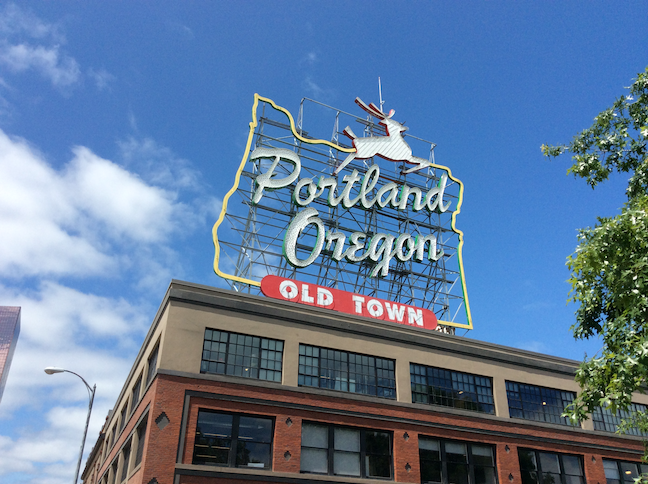
\includegraphics[height=1.75cm]{portland}};
\node[inner sep=0pt] (applekameraicon) at (0,0) {
\includegraphics[scale=0.1]{apple-kamera-icon}};
\node[inner sep=0pt] (smartphonefestplatte) at (5,0) {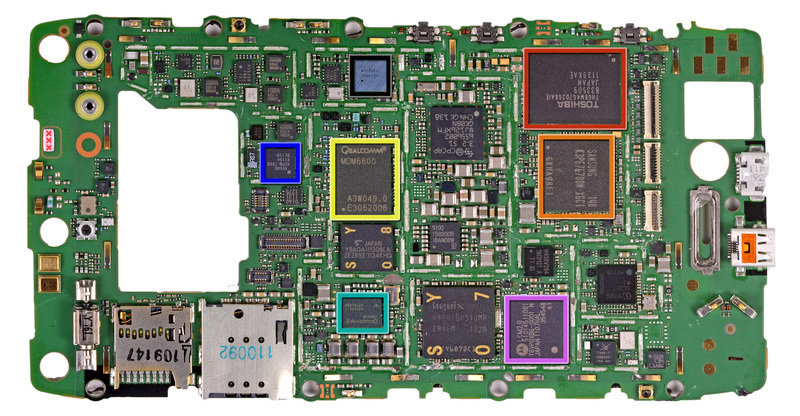
\includegraphics[height=1.75cm]{smartphone_festplatte}};
\draw[-latex, thick] (portland) -- (applekameraicon) node[midway, fill=white] {\say{Klick}};
\draw[-latex, thick] (applekameraicon) -- (smartphonefestplatte) node[midway, fill=white] {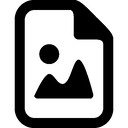
\includegraphics[scale=0.15]{image_file_icon}};
\end{tikzpicture}
\caption{Das Bild zwischen Kamera-App und Platine\protect\footnotemark~mit Computerchips stellt die Bilddatei dar. Die rote Box kennzeichnet den internen Speicher des Smartphones.}
\label{figure-informationsspeicherung}
\end{figure}

\footnotetext{Eine Platine (auch Leiterplatte genannt) ist ein Träger für elektronische Bauteile wie zum Beispiel Computerchips.}

Das Bild stellt hier die Information dar, welche in einer Bilddatei gespeichert wird.

\begin{definition}[Datei]
In einer Datei (engl. file) kann ein Computer Daten langfristig auf einem Speichermedium (Festplatte, USB-Stick, Smartphone-Speicher etc.) unter einem Namen speichern. Die gespeicherten Informationen in der Datei können sehr vielseitig sein: Texte, Bilder, Audio, Video, \dots . Dateien bleiben nach einem Neustart des Computers erhalten und werden nicht gelöscht.
\end{definition}

\begin{definition}[Bilddatei]
Eine Datei, in der ein Bild gespeichert ist, nennen wir Bilddatei.
\end{definition}

\begin{definition}[Dateinamen-Erweiterung]
Ein Dateiname wird unter Verwendung eines Punktes (\texttt{.}) in zwei Teile gegliedert, den eigentlichen Namen und die sogenannte Dateinamen-Erweiterung (engl. file extension).
\end{definition}

\begin{example}
Es gibt zahlreiche Dateinamen-Erweiterungen. Hier ein paar bekannte Beispiele:
\begin{itemize}
\item Für Word-Dateien gibt es die Dateinamen-Erweiterung \texttt{.docx}.
\item Für Bilddateien gibt es zum Beispiel die Dateinamen-Erweiterung \texttt{.png}, \texttt{.jpg} oder \texttt{.gif}.
\item Für PDF-Dateien gibt es die Dateinamen-Erweiterung \texttt{.pdf}.
\item Für PowerPoint-Dateien gibt es die Dateinamen-Erweiterung \texttt{.pptx}.
\end{itemize}
Ein vollständiger Dateiname wäre zum Beispiel \texttt{portland.jpg}.
\end{example}

Wir klären in diesem Skript, wie der Computer in einer Datei ein Bild oder Text speichert.

\section{Reduktion der Datengrösse}

Jede Datei auf der Festplatte beansprucht Speicherplatz. Nimmt man ein Foto mit dem Smartphone auf, dann wird eine Bilddatei erzeugt. Diese Bilddateien besitzen in der Regel eine Grösse zwischen \qty{2}{\mega\byte} und \qty{3}{\mega\byte}. Auch Textdateien wie zum Beispiel eine Word-Datei besitzen eine gewisse Grösse. Da in den letzten Jahren immer mehr Daten produziert und gespeichert werden (Stichwort \say{Big Data}) ist man daran interessiert, den Speicherplatz möglichst effizient zu nutzen. Dies kann man dadurch erreichen, indem man Verfahren einsetzt, welche die Datengrösse etwa von Bildern reduziert. Warum sollte man die Datengrösse überhaupt reduzieren?

\begin{itemize}
\item Der Speicherplatz auf der Festplatte oder dem Smartphone-Speicher ist begrenzt. Ohne eine Reduktion der Dateigrösse wäre der Speicherplatz noch schneller voll.
\item Die Übertragungsdauer von Daten im Internet kann durch eine Reduktion der Datengrösse verbessert werden.
\end{itemize}

\begin{figure}[htb]
\centering
\begin{minipage}{0.45\textwidth}
\centering
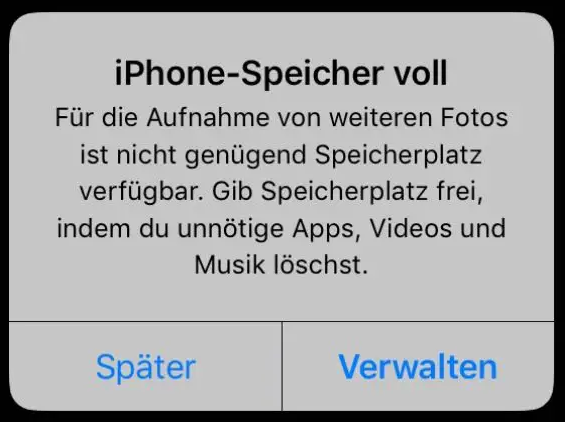
\includegraphics[height=4cm]{iphone_speicher_voll}
\end{minipage}
\begin{minipage}{0.45\textwidth}
\centering
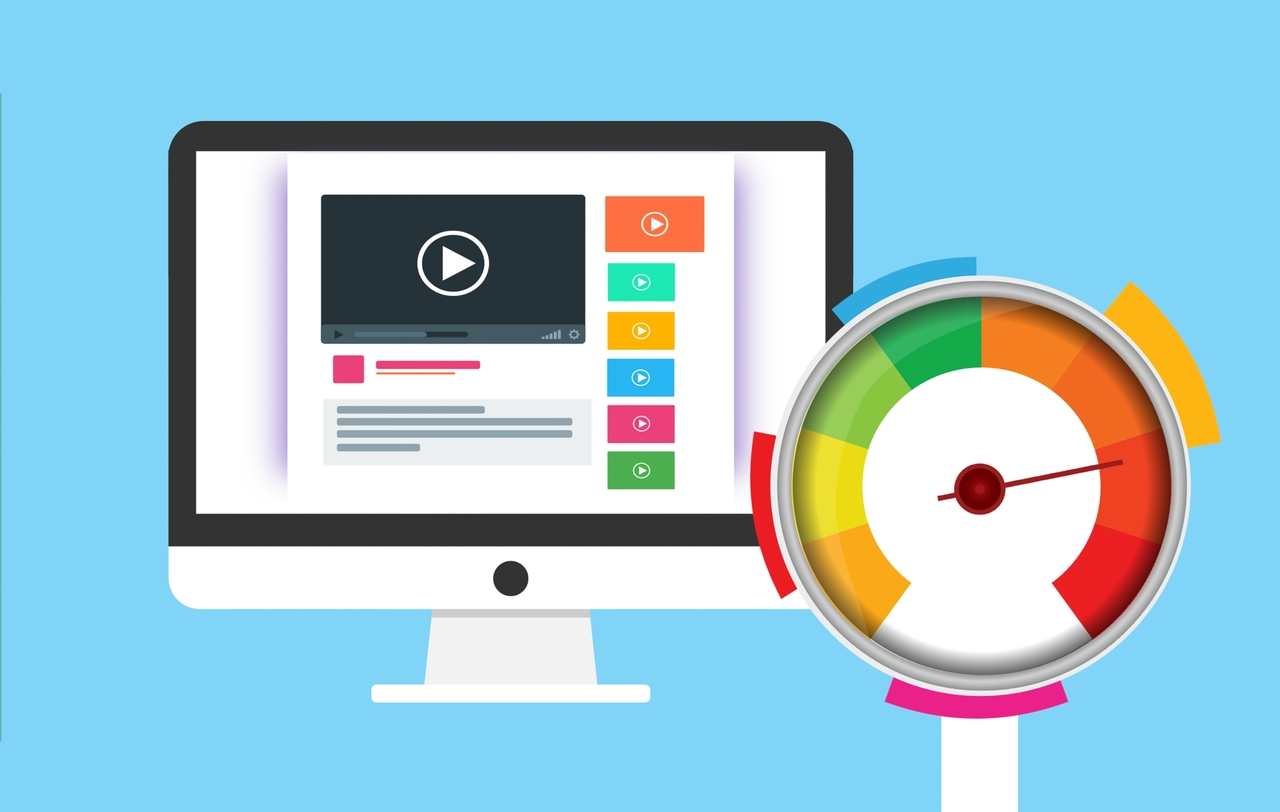
\includegraphics[height=4cm]{internet_speed}
\end{minipage}
\end{figure}

Einige Bilddateien verwenden automatisch eine Technik, um die Datengrösse zu reduzieren. Auch bei WhatsApp werden die Bilder in der Standardeinstellung nicht in der besten Qualität verschickt. Ohne die Verfahren zur Reduktion der Datengrösse wäre das \say{Surfen} im World Wide Web deutlich mühsamer, wenn nicht gar undenkbar. Die Ladezeiten von Websites wären teilweise unerträglich hoch. Wir möchten in diesem Skript deshalb die Grundlagen zur Reduktion der Datengrösse kennenlernen.

\newpage

\section{Fehlererkennung und Fehlerkorrektur bei der Datenübertragung}

Bei der Datenübertragung schickt ein Sender eine Nachricht an einen Empfänger (\autoref{figure-datenübertragung}). Dies kann zum Beispiel eine WhatsApp-Nachricht sein. Dabei verschickt der Computer ganz automatisch die für die Nachricht notwendigen Daten vom Sender-Gerät zum Empfänger-Gerät. 

\begin{figure}[htb]
\centering
\begin{tikzpicture}
\node[inner sep=0pt] (sender) at (-5,0) {
\includegraphics[height=2cm]{lego_alice}};
\node[inner sep=0pt] (empfaenger) at (5,0) {
\includegraphics[height=2cm]{lego_bob}};
\node[below=0.5cm of sender] {Sender (Alice)};
\node[below=0.5cm of empfaenger] {Empfänger (Bob)};
\node[inner sep=0pt, red] (fehler) at (0,-1) {Fehler};
\draw[-latex, thick] (sender) -- (empfaenger) node[midway, fill=white] {\say{Datenübertragung}};
\draw[-latex, thick, red] (fehler) -- (0,-0.1);
\end{tikzpicture}
\caption{Sender schickt eine Nachricht an den Empfänger. Bei der Übertragung passiert ein Fehler. Besteht die Nachricht aus dem Wort Hose, dann könnte zum Beispiel durch einen Übertragungsfehler beim Empfänger das Wort Hase ankommen.}
\label{figure-datenübertragung}
\end{figure}


Die Ursachen für Fehler bei der Datenübertragung können vielseitig sein. Ein paar Beispiele:

\begin{itemize}
\item Physikalische Effekte (Elektronenbewegung in Leitungen, elektromagnetische oder radioaktive Einstrahlung)
\item Schadhafte Geräte (Spannung oder Kontakte sind defekt)
\item Hohe Last im Netzwerk (z.B. \ac{WLAN})
\end{itemize}

Als Folge können die Daten inkorrekt am Empfänger ankommen oder verloren gehen (teilweise oder vollständig). Wir schauen uns in diesem Skript einfache Verfahren an, wie man einen Fehler bei der Datenübertragung erkennen und korrigieren kann. Wir untersuchen also nur den Fall, dass die Daten ankommen, jedoch während der Übertragung (unabsichtlich) verändert wurden. 